% ============================================================
\section{Abstrakce OS: procesy, vlákna, plánování a soubory}
% ============================================================

Operační systém staví nad holým hardwarem dvě klíčové \emph{abstrakce sdílení prostředků}: sdílení \emph{procesoru} (aby se zdálo, že má každá běžící úloha procesor sama pro sebe -- procesy a vlákna) a sdílení \emph{úložného prostoru} (pojmenované soubory). Tato sekce zavádí procesy, vlákna, kontext a jeho přepínání, plánování a stavy plánovací jednotky a krátce souborovou abstrakci. Vychází z~režimů procesoru a~jádra ze sekce~3; \emph{sdílení paměti a~virtuální paměť} (adresový prostor jako mapování VA$\to$FA, stránkování) řeší samostatně sekce~6.

\subsection{Proces a vlákno}

\begin{definice}[Program, proces, vlákno]
\emph{Program} je \emph{pasivní} sada instrukcí a~dat (soubor na disku, výstup překladače). \emph{Proces} je \emph{instance} programu vytvořená OS za běhu: dostane vlastní \emph{adresový prostor} (paměť) a~vlastní \emph{prostředky} (otevřené soubory, sokety, synchronizační primitiva). Proces v~podstatě poskytuje aplikaci virtuální stroj. \emph{Vlákno} (thread) je \emph{jeden tok instrukcí} (jedna aktivita) vykonávaný procesorem uvnitř procesu; je to \emph{jednotka plánování}. Každý proces má aspoň jedno vlákno, může jich mít víc.
\end{definice}

\begin{intuice}
Hranice „co je čí`` je důležitá. Vlákno má \emph{vlastní} jen to, co je nutné k~jeho samostatnému běhu: pozici v~kódu (program counter), \emph{zásobník} (stack -- lokální proměnné a~návratové adresy) a~\emph{stav procesoru} (obsah registrů). Všechno ostatní -- kód, statická data, halda, otevřené soubory -- vlákna procesu \emph{sdílejí}. Proto je komunikace mezi vlákny levná (sdílená paměť), ale vyžaduje synchronizaci (sekce~7), zatímco procesy jsou navzájem izolované.
\end{intuice}

\begin{definice}[Neprivilegovaný (uživatelský) proces]
\emph{Neprivilegovaný} (uživatelský) proces běží v~\emph{uživatelském režimu} procesoru (sekce~3): nemá přímý přístup k~hardwaru ani k~paměti jádra a~ostatních procesů a~o~privilegované operace musí žádat jádro \emph{systémovým voláním} (syscall). Adresové prostory procesů jsou navzájem oddělené, takže chyba či zlovolný kód jednoho procesu nemůže přímo poškodit ostatní. Tato \emph{izolace} je základní bezpečnostní a~spolehlivostní vlastnost OS.
\end{definice}

\subsection{Kontext a přepínání kontextu}

\begin{definice}[Kontext plánovací jednotky]
\emph{Kontext} je stav plánovací jednotky (vlákna, resp.\ procesu), který OS musí uchovat, aby šel její běh později přesně obnovit. Patří do něj:
\begin{itemize}
\item \emph{obsah registrů procesoru} -- včetně program counteru (IP/PC), stack pointeru (SP), stavového slova (příznaky), případně vektorových a~FP registrů;
\item \emph{stav virtuální paměti} -- ukazatel na stránkovací tabulky a~obsah TLB (podrobně sekce~6); ten se přepíná při změně \emph{procesu}, ne mezi vlákny téhož procesu, která adresový prostor sdílejí.
\end{itemize}
Cache jsou \emph{transparentní} -- nejsou součástí kontextu (jen ovlivní výkon).
\end{definice}

\begin{definice}[Přepnutí kontextu (context switch)]
\emph{Přepnutí kontextu} je operace, při níž OS \emph{uloží} kontext právě běžící jednotky (do její struktury v~jádře) a~\emph{obnoví} kontext jiné jednotky, kterou nasadí na procesor. Je to \emph{drahá} operace (řádově stovky až tisíce instrukcí): kromě uložení a~obnovy registrů zahrnuje u~změny procesu i~přepnutí adresového prostoru, což (bez ASID, sekce~6) zneplatní položky v~TLB (a~znovunaplnění TLB stojí další přístupy do paměti).
\end{definice}

\subsection{Multitasking: kooperativní vs. preemptivní}

\emph{Multitasking} je souběžný (concurrent) běh více úloh na (případně jediném) procesoru tak, že se o~něj střídají. Liší se podle toho, \emph{kdo a~kdy} rozhodne o~odebrání procesoru běžící jednotce.

\begin{definice}[Kooperativní vs. preemptivní multitasking]
Při \emph{kooperativním} multitaskingu se běžící jednotka musí procesoru vzdát \emph{sama a~dobrovolně} (vrátí řízení OS, typicky voláním \emph{yield} nebo zablokováním na I/O). OS sám běh nepřeruší, takže jediná nekooperující jednotka může zablokovat celý systém. Při \emph{preemptivním} multitaskingu má každá běžící jednotka přidělené \emph{časové kvantum} (time slice); když je vyčerpá, \emph{hardwarový časovač} vyvolá přerušení, OS dostane řízení a~jednotku \emph{preempuje} (odebere jí procesor, přepne na jinou). Preempce tak nevyžaduje spolupráci úloh a~zaručuje spravedlivé sdílení -- proto ji používají moderní OS pro obecné výpočty.
\end{definice}

\begin{poznamka}
Pokud se jednotka v~preemptivním režimu zablokuje nebo skončí ještě před vypršením kvanta, časovač není potřeba -- OS přepne hned. Kooperativní model se dnes vyskytuje spíš uvnitř běhových prostředí (např.\ uživatelská vlákna / \emph{fibery} a~asynchronní úlohy s~explicitním \emph{await}).
\end{poznamka}

\subsection{Plánování (scheduling)}

\emph{Plánovač} (scheduler) je část OS, která pomocí \emph{plánovacích algoritmů} rozhoduje, která připravená jednotka poběží na procesoru (jádře). Volí kompromis mezi několika cíli:

\begin{definice}[Cíle plánování]
\emph{Využití procesoru} (utilization) -- udržet procesor co nejvíc vytížený. \emph{Propustnost} (throughput) -- počet úloh dokončených za jednotku času. \emph{Obrátková doba} (turnaround) -- celkový čas od příchodu úlohy do jejího dokončení. \emph{Čekací doba} (waiting time) -- čas strávený ve stavu \emph{Ready} (čekáním na procesor). \emph{Doba odezvy} (response time) -- čas do první reakce u~interaktivních aplikací. K~tomu \emph{spravedlnost} (fairness). Cíle jsou často protichůdné (např.\ krátká odezva vs.\ vysoká propustnost).
\end{definice}

\begin{definice}[Základní plánovací algoritmy]
\emph{FCFS} (First Come, First Served) -- jediná FIFO fronta; jednotky běží v~pořadí příchodu a~\emph{bez přerušení} až do konce (nepreemptivní). Jednoduché, ale dlouhá úloha vepředu zdrží všechny za sebou (konvojový efekt).\\
\emph{SJF} (Shortest Job First) -- přednost dostane úloha s~\emph{nejkratší} dobou běhu; při současném příchodu úloh minimalizuje průměrnou čekací dobu, ale vyžaduje znát (či odhadnout) délku úloh předem.\\
\emph{Round Robin} (RR) -- jako FCFS, ale \emph{preemptivní}: každá jednotka dostane časové kvantum; když ho vyčerpá (nebo se zablokuje), zařadí se na \emph{konec} fronty a~procesor dostane další. Malé kvantum dává krátkou odezvu, ale víc přepnutí kontextu (režie).\\
\emph{Víceúrovňová fronta se zpětnou vazbou} (multilevel feedback queue) -- několik front s~rostoucím kvantem; jednotka, která vyčerpá celé kvantum, klesne do nižší (méně časté) fronty, jednotka, která se zablokuje dřív (interaktivní, I/O-vázaná), stoupne do vyšší. Plánuje se vždy hlava nejvyšší neprázdné fronty. Tak se interaktivní úlohy zvýhodní bez znalosti jejich délky předem.
\end{definice}

\begin{definice}[Priorita]
\emph{Priorita} je číslo vyjadřující důležitost jednotky; jednotka s~vyšší prioritou se plánuje dřív (nebo častěji). Typicky jde o~součet \emph{statické priority} (přidělené při startu podle důležitosti uživatele/úlohy) a~\emph{dynamické priority}, která přidává spravedlnost: OS ji čas od času zvyšuje všem čekajícím (\emph{Ready}) jednotkám a~nuluje ji té, která byla právě naplánována -- aby dlouho čekající úloha nezůstala „vyhladovělá``.
\end{definice}

\begin{poznamka}
Linux dnes plánuje implementačně propracovaným algoritmem (dříve \emph{CFS}, jednotky v~červeno-černém stromě indexované nasčítaným časem běhu, plánuje se nejméně využitá). Konkrétní detaily těchto algoritmů jdou nad rámec požadavků okruhu.
\end{poznamka}

\subsection{Stavy plánovací jednotky}

Vlákno (proces) prochází během života několika \emph{stavy}; přechody mezi nimi vyvolávají události v~systému (plánovač, časovač, dostupnost prostředku).

\begin{definice}[Stavy a přechody]
\emph{Created} (vytvořen) -- jednotka vznikla, čeká na přijetí (admission) plánovačem. \emph{Ready} (připraven) -- je připravená běžet a~čeká \emph{jen na procesor}. \emph{Running} (běžící) -- má přidělený procesor a~vykonává instrukce. \emph{Blocked} (čeká/spí) -- čeká na \emph{prostředek} (dokončení I/O, uvolnění zámku, příchod dat), a~tak nemůže pokračovat, ani kdyby procesor dostala. \emph{Terminated} (ukončen) -- doběhla; drží se (jako „zombie``), dokud rodič nepřevezme návratový kód. Hlavní přechody: \emph{admit} Created$\to$Ready, \emph{dispatch} Ready$\to$Running, \emph{preempce/vypršení kvanta} Running$\to$Ready, \emph{block/wait} Running$\to$Blocked, \emph{wakeup} (prostředek k~dispozici) Blocked$\to$Ready, \emph{exit} Running$\to$Terminated.
\end{definice}

\begin{center}
\scalebox{1.2}{%
\begin{tikzpicture}[>=Stealth]
% rozmisteni: Created vlevo nahore, Ready vlevo dole, Running vpravo nahore,
% Blocked vpravo dole, Terminated vpravo nahore nad Running
\node[stav] (created)    at (0,2.6)  {Created};
\node[stav] (ready)      at (0,0)    {Ready};
\node[stav] (running)    at (5,2.6)  {Running};
\node[stav] (blocked)    at (5,0)    {Blocked};
\node[stav] (terminated) at (9.2,2.6){Terminated};
% hrany s popisky na uzlech (gotchas: align na uzel)
\draw[flow] (created) -- node[font=\scriptsize,midway,right,align=left]{admit} (ready);
\draw[flow] (ready.east) to[bend left=22]
  node[font=\scriptsize,pos=0.5,above=1pt]{dispatch} (running.west);
\draw[flow] (running.west) to[bend left=22]
  node[font=\scriptsize,pos=0.5,below=1pt]{preempce} (ready.east);
\draw[flow] (running) -- node[font=\scriptsize,midway,right,align=left]{block / wait\\(čeká na prostředek)} (blocked);
\draw[flow] (blocked) -- node[font=\scriptsize,midway,below,align=center]{wakeup\\(prostředek k~dispozici)} (ready);
\draw[flow] (running) -- node[font=\scriptsize,midway,above,align=center]{exit} (terminated);
\end{tikzpicture}}%
\obrpopis{Stavy plánovací jednotky a~přechody. Rozdíl \emph{Blocked} vs.\ \emph{Ready} je klíčový: jednotka v~\emph{Blocked} čeká na \emph{prostředek} (typicky dokončení I/O nebo uvolnění zámku) a~plánovač jí procesor nepřidělí, dokud prostředek nedorazí (přechod \emph{wakeup}); jednotka v~\emph{Ready} je k~běhu plně připravená a~čeká \emph{jen} na to, až ji plánovač nasadí na procesor. Plánuje se vždy mezi jednotkami ve stavu \emph{Ready}.}
\end{center}

\subsection{Adresový prostor procesu (kde leží zásobníky vláken)}

Než přejdeme k~souborům, shrňme rozvržení \emph{adresového prostoru} procesu -- ukazuje, co vlákna sdílejí a~co má každé vlastní. (Detailní mechanismus mapování na fyzickou paměť je v~sekci~6.)

\begin{center}
\scalebox{1.15}{%
\begin{tikzpicture}[y=0.5cm,every node/.append style={font=\footnotesize}]
% y-jednotka = 1; bloky odshora (nizke adresy nahore) dolu (vysoke adresy dole)
% poradi: Kod, Konstanty, Init. data, Neinit. data, [volne], Halda, ..., Zasobniky vlaken
% Kreslime shora dolu: nahore nizke adresy. Halda roste dolu od svého zacatku,
% zasobniky rostou nahoru od vysokych adres. Zde: text nahore, zasobniky dole.
\def\W{4.0}
% bloky (y odshora): kazdy vysoky 2 jednotky
\fill[blue!7]  (0,16) rectangle (\W,18); \draw (0,16) rectangle (\W,18);
\fill[blue!7]  (0,14) rectangle (\W,16); \draw (0,14) rectangle (\W,16);
\fill[blue!7]  (0,12) rectangle (\W,14); \draw (0,12) rectangle (\W,14);
\fill[blue!7]  (0,10) rectangle (\W,12); \draw (0,10) rectangle (\W,12);
% halda (roste dolu)
\fill[green!10](0,7)  rectangle (\W,10); \draw (0,7)  rectangle (\W,10);
% volne misto
\fill[black!3] (0,4)  rectangle (\W,7);  \draw[dashed] (0,4) rectangle (\W,7);
% zasobniky vlaken (rostou nahoru)
\fill[red!8]   (0,2)  rectangle (\W,4);  \draw (0,2)  rectangle (\W,4);
\fill[red!8]   (0,0)  rectangle (\W,2);  \draw (0,0)  rectangle (\W,2);
% popisky bloku
\node at (\W/2,17) {Kód (instrukce)};
\node at (\W/2,15) {Konstanty};
\node at (\W/2,13) {Inicializovaná stat.\ data};
\node at (\W/2,11) {Neinicializ.\ stat.\ data};
\node at (\W/2,8.5){Halda};
\node at (\W/2,5.5){\textit{(volné místo)}};
\node at (\W/2,3) {Zásobník vlákna~1};
\node at (\W/2,1) {Zásobník vlákna~$n$};
\node[font=\scriptsize] at (\W/2,2.4) {$\vdots$};
% sipky rustu
\draw[ptr,green!45!black] (\W+0.35,9.7) -- (\W+0.35,7.3)
  node[midway,right,font=\scriptsize,green!45!black,align=left]{halda roste dolů\\(k~vyšším adr.)};
\draw[ptr,red!60!black]   (\W+0.35,2.3) -- (\W+0.35,3.9)
  node[midway,right,font=\scriptsize,red!60!black,align=left]{zásobníky rostou\\nahoru (k~nižším adr.)};
% popisky nizke/vysoke adresy
\node[anchor=east,font=\scriptsize] at (-0.15,17.5) {nízké adresy};
\node[anchor=east,font=\scriptsize] at (-0.15,0.5)  {vysoké adresy};
% zavorka: sdilene oblasti
\draw[decorate,decoration={brace,amplitude=5pt}] (-1.05,10) -- (-1.05,18)
  node[midway,anchor=east,shift={(-0.2,0)},font=\scriptsize,align=center]{sdílí\\všechna\\vlákna};
\draw[decorate,decoration={brace,amplitude=5pt}] (-1.05,0) -- (-1.05,4)
  node[midway,anchor=east,shift={(-0.2,0)},font=\scriptsize,align=center]{per\\vlákno};
\end{tikzpicture}}%
\obrpopis{Adresový prostor procesu. Oblasti \emph{kód}, \emph{konstanty}, \emph{inicializovaná} a~\emph{neinicializovaná statická data} a~\emph{halda} (dynamicky alokovaná paměť, viz sekce~1) jsou pro celý proces \emph{sdílené} mezi vlákny. Naproti tomu \emph{každé vlákno má vlastní zásobník} (lokální proměnné a~návratové adresy), protože každé vykonává svou vlastní posloupnost volání. Halda typicky roste směrem k~vyšším adresám, zásobníky opačně; mezi nimi je volné místo, do kterého obě strany expandují.}
\end{center}

\subsection{Soubory: sdílení úložného prostoru}

Druhou velkou abstrakcí je sdílení \emph{úložného prostoru}. OS skrývá rozmanitost médií (disk, SSD, síť) za jednotný pojem souboru.

\begin{definice}[Soubor]
\emph{Soubor} (file) je pojmenovaná jednotka organizace dat -- z~pohledu jádra \emph{abstraktní proud (posloupnost) bajtů}. Jádro \emph{nerozumí} formátu obsahu (to je věc aplikace), vidí jen lineární sled bajtů a~jejich délku. Soubor identifikuje OS \emph{číselným} identifikátorem; \emph{jméno a~cesta} (ve stromové struktuře adresářů) jsou jen lidsky čitelný odkaz na tento identifikátor.
\end{definice}

\begin{intuice}[Analogie s adresovým prostorem]
Soubor je vůči datům na disku tím, čím je adresový prostor vůči paměti: \emph{lineární, od nuly adresovatelná posloupnost bajtů}. Místo „adresy`` se v~souboru pohybujeme \emph{pozicí} (offsetem) a~podobně jako u~paměti čteme/zapisujeme souvislé úseky od dané pozice. Operace \emph{seek} (nastavení pozice) je analogie skoku na adresu, sekvenční čtení je analogie procházení paměti po sobě jdoucími adresami. OS tak nabízí jeden jednotný způsob „náhodného přístupu k~bajtům`` jak pro paměť, tak pro úložiště.
\end{intuice}

\begin{definice}[Rozhraní pro práci se soubory]
Základní operace (POSIX): \emph{open} -- otevře soubor podle jména, vrátí \emph{deskriptor}; \emph{read}/\emph{write} -- přečte/zapíše daný počet bajtů od aktuální pozice (a~pozici posune); \emph{seek} (lseek) -- nastaví aktuální pozici v~souboru; \emph{close} -- soubor zavře a~uvolní deskriptor. Doplňkové operace: \emph{create}, \emph{truncate}, \emph{delete}, \emph{flush}, změna atributů.
\end{definice}

\begin{definice}[File handle / deskriptor]
\emph{File handle} (deskriptor) je číselný identifikátor otevřeného souboru, \emph{lokální pro proces} a~přidělovaný postupně. Jádro k~němu vede \emph{překladovou tabulku} (deskriptor $\to$ vnitřní stav otevřeného souboru: o~který soubor jde a~jaká je aktuální pozice). Aplikace tedy pracuje jen s~malým celým číslem, skutečnou vazbu na soubor drží jádro. První tři deskriptory má proces po startu otevřené z~konvence: \textbf{0~= stdin} (standardní vstup), \textbf{1~= stdout} (standardní výstup), \textbf{2~= stderr} (chybový výstup).
\end{definice}

\begin{poznamka}
Mezi \emph{open} a~\emph{read}/\emph{write} se kvůli výkonu vkládá \emph{vyrovnávací paměť} (buffering) na více úrovních (jádro, běhové prostředí). Jak je soubor skutečně \emph{uložen} na médiu (souborové systémy FAT, ext, adresáře, bloky) je už věc implementace souborového systému a~jde nad rámec tohoto okruhu -- nás zajímá souborová \emph{abstrakce a~rozhraní}.
\end{poznamka}

\subsection{Řešený příklad: plánování Round Robin}

\begin{priklad}[Round Robin -- Ganttův diagram, obrátková a čekací doba]
\textbf{Zadání.}\par
Tři procesy přijdou všechny v~čase $0$ s~dobami běhu \mbox{$P_1=5$}, \mbox{$P_2=3$}, \mbox{$P_3=3$} (v~jednotkách času). Plánuje se algoritmem \emph{Round Robin} s~kvantem $q=2$; ve frontě připravených jsou na začátku v~pořadí $P_1,P_2,P_3$. Sestrojte Ganttův diagram pořadí běhu a~spočítejte pro každý proces \emph{obrátkovou} dobu (turnaround $=$ dokončení $-$ příchod) a~\emph{čekací} dobu (waiting $=$ obrátková $-$ doba běhu).

\medskip
\textbf{Řešení.}\par
Každý proces běží nejvýš $q=2$ jednotky, pak (pokud nedoběhl) jde na konec fronty. Procesy přišly v~čase $0$, takže se po preempci vracejí na konec aktuální fronty. Zbývající doby běhu a~průběh fronty:
\begin{enumerate}
\item $[0,2]$: běží $P_1$ (zbývá $5\to3$), na konec. Fronta: $P_2,P_3,P_1$.
\item $[2,4]$: běží $P_2$ (zbývá $3\to1$), na konec. Fronta: $P_3,P_1,P_2$.
\item $[4,6]$: běží $P_3$ (zbývá $3\to1$), na konec. Fronta: $P_1,P_2,P_3$.
\item $[6,8]$: běží $P_1$ (zbývá $3\to1$), na konec. Fronta: $P_2,P_3,P_1$.
\item $[8,9]$: běží $P_2$ (zbývá $1\to0$), \textbf{dokončen v~čase~9}. Fronta: $P_3,P_1$.
\item $[9,10]$: běží $P_3$ (zbývá $1\to0$), \textbf{dokončen v~čase~10}. Fronta: $P_1$.
\item $[10,11]$: běží $P_1$ (zbývá $1\to0$), \textbf{dokončen v~čase~11}.
\end{enumerate}

\begin{center}
\scalebox{1.2}{%
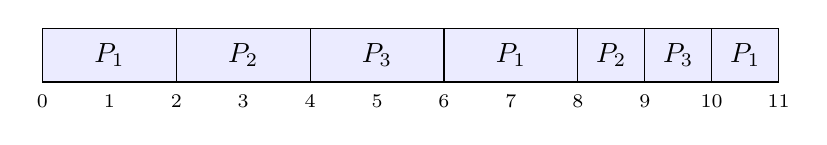
\begin{tikzpicture}[x=0.85cm,y=0.85cm]
% Ganttuv diagram: rada bunek na case 0..11
% segmenty: P1 0-2, P2 2-4, P3 4-6, P1 6-8, P2 8-9, P3 9-10, P1 10-11
\foreach \a/\b/\p in {0/2/1, 2/4/2, 4/6/3, 6/8/1, 8/9/2, 9/10/3, 10/11/1} {
  \draw[fill=blue!8] (\a,0) rectangle (\b,0.8);
  \node at ({(\a+\b)/2},0.4) {$P_{\p}$};
}
% casova osa
\foreach \t in {0,...,11}
  \node[anchor=north,font=\scriptsize] at (\t,-0.05) {\t};
\draw[thick] (0,0) -- (11,0);
\end{tikzpicture}}%
\obrpopis{Ganttův diagram běhu Round Robin ($q=2$). Procesy se o~procesor střídají po kvantech; $P_2$ a~$P_3$ doběhnou v~poslední polovině (kratší zbytky $1$), $P_1$ s~nejdelší dobou běhu doběhne až úplně poslední v~čase~11.}
\end{center}

Dokončení: $P_1$ v~$11$, $P_2$ v~$9$, $P_3$ v~$10$. Příchod všech $=0$, takže obrátková doba $=$ čas dokončení a~čekací $=$ obrátková $-$ doba běhu:
\begin{center}
\begin{tabular}{c|c|c|c|c}
proces & doba běhu & dokončení & obrátková & čekací\\\hline
$P_1$ & $5$ & $11$ & $11$ & $11-5=\boxed{6}$\\
$P_2$ & $3$ & $9$  & $9$  & $9-3=\boxed{6}$\\
$P_3$ & $3$ & $10$ & $10$ & $10-3=\boxed{7}$\\
\end{tabular}
\end{center}
Průměrná obrátková doba je $\tfrac{11+9+10}{3}=\boxed{10}$, průměrná čekací doba $\tfrac{6+6+7}{3}=\tfrac{19}{3}\approx\boxed{6{,}33}$. Kontrola: součet všech dob běhu je $5+3+3=11$, což přesně sedí s~okamžikem, kdy doběhl poslední proces (procesor nikdy nezahálel). \textit{(Ilustrativní příklad; Ganttův diagram i~doby ověřeny simulací RR v~Pythonu.)}
\end{priklad}
